\chapter{S\`{e}ries de Fourier}\label{sec:serie_fu} \index{s\`{e}ries de
Fourier}\index{Fourier, s\`{e}ries de}

\section{Definicions}\index{s\`{e}ries de Fourier!definicions}

Una funci\'{o} peri\`{o}dica en el temps $v(t)$, de freq\"{u}\`{e}ncia $f$, per\'{\i}ode
$T$ i velocitat angular $\omega$ ($f = 1/T$, $\omega=2\pi f =
2\pi/T$), es pot expressar com una suma infinita de funcions sinus i
cosinus; \'{e}s el que s'anomena expansi\'{o} d'una funci\'{o} peri\`{o}dica en
s\`{e}rie de Fourier:
\begin{equation}
    v(t) = A_0 + \sum_{n=1}^\infty A_n \cos (n \omega t) +
    \sum_{n=1}^\infty B_n \sin (n \omega t) \label{eq:serie_fu_wt}
\end{equation}

Els coeficients $A_0$, $A_n$ i $B_n$, es calculen a partir de les
expressions seg\"{u}ents:
\begin{subequations}
\begin{alignat}{3}
    A_0 &= \frac{1}{T} \int_{t_0}^{t_0+T} v(t) \diff t &&=
    \frac{\omega}{2\pi} \int_{t_0}^{t_0+\frac{2\pi}{\omega}} v(t) \diff
    t \label{eq:a0_t} & \\[0.5ex]
    A_n &= \frac{2}{T} \int_{t_0}^{t_0+T} v(t) \cos(n \omega t) \diff
    t &&=
    \frac{\omega}{\pi} \int_{t_0}^{t_0+\frac{2\pi}{\omega}} v(t)\cos(n \omega t) \diff
    t &\qquad(n=1,\ldots\infty)\\[0.5ex]
    B_n &= \frac{2}{T} \int_{t_0}^{t_0+T} v(t) \sin(n \omega t) \diff t
    &&=
    \frac{\omega}{\pi} \int_{t_0}^{t_0+\frac{2\pi}{\omega}} v(t)\sin(n \omega t) \diff
    t &\qquad(n=1,\ldots\infty)
\end{alignat}
\end{subequations}

Si la funci\'{o} peri\`{o}dica $v(\alpha)$ est\`{a} definida en funci\'{o} de
l'angle $\alpha$, enlloc del temps $t$, a partir de la relaci\'{o}
$\alpha=\omega t$ ($\diff\alpha=\omega\diff t$), tenim:
\begin{equation}
    v(\alpha) = A_0 + \sum_{n=1}^\infty A_n \cos n \alpha +
    \sum_{n=1}^\infty B_n \sin n \alpha \label{eq:serie_fu_alfa}
\end{equation}

En aquest cas, els coeficients $A_0$, $A_n$ i $B_n$, es calculen a
partir de les expressions seg\"{u}ents:
\begin{subequations}
\begin{alignat}{2}
    A_0 &= \frac{1}{2\pi} \int_{\alpha_0}^{\alpha_0+2\pi} v(\alpha) \diff \alpha
    \label{eq:a0_alfa} & \\[0.5ex]
    A_n &= \frac{1}{\pi} \int_{\alpha_0}^{\alpha_0+2\pi} v(\alpha) \cos n \alpha \diff
    \alpha &\qquad(n=1,\ldots\infty)\\[0.5ex]
    B_n &= \frac{1}{\pi} \int_{\alpha_0}^{\alpha_0+2\pi} v(\alpha) \sin n \alpha \diff \alpha
    &\qquad(n=1,\ldots\infty)
\end{alignat}
\end{subequations}

Les equacions \eqref{eq:serie_fu_wt} i \eqref{eq:serie_fu_alfa}, es
poden expressar d'una manera alternativa, utilitzant \'{u}nicament
funcions cosinus:
\begin{align}
    v(t) &= C_0 + \sum_{n=1}^\infty C_n \cos (n \omega t + \phi_n)
    \label{eq:serie_f_c_t}\\[0.5ex]
    v(\alpha) &= C_0 + \sum_{n=1}^\infty C_n \cos (n \alpha +
    \phi_n)\label{eq:serie_f_c_alfa}
\end{align}

Els coeficients $C_0$, $C_n$ i $\phi_n$, es calculen a partir de les
expressions seg\"{u}ents:
\begin{subequations}
\begin{alignat}{2}
    C_0 &= A_0 & \\[0.5ex]
    C_n &= \sqrt{A_n^2+B_n^2} &\qquad(n=1,\ldots\infty)\\[0.5ex]
    \phi_n &= -\arctan \frac{B_n}{A_n} &\qquad(n=1,\ldots\infty)
\end{alignat}
\end{subequations}

Si comparem l'equaci\'{o} \eqref{eq:a0_t} amb l'equaci\'{o} \eqref{eq:vm_t}
o l'equaci\'{o} \eqref{eq:a0_alfa} amb l'equaci\'{o} \eqref{eq:vm_alfa},
veurem que s\'{o}n id\`{e}ntiques, per tant, es pot afirmar que el
coeficient $A_0$ (i per tant $C_0$) \'{e}s igual al valor mitj\`{a} de la
funci\'{o} peri\`{o}dica.

Atenent a les equacions  \eqref{eq:serie_f_c_t} o
\eqref{eq:serie_f_c_alfa}, el terme d'\'{\i}ndex $n=1$, $C_1 \cos (\omega
t + \phi_1)$ o $C_1 \cos (\alpha + \phi_1)$,  s'anomena component
fonamental, perqu\`{e} t\'{e} la mateixa freq\"{u}\`{e}ncia que la funci\'{o} original.
La resta de termes, d'\'{\i}ndex $n=2,\ldots,\infty$, s'anomenen
components harm\`{o}niques.

\section{Simplificacions}\index{s\`{e}ries de Fourier!simplificacions}

Quan les funcions $v(t)$ o $v(\alpha)$ presenten certes simetries,
alguns dels coeficients $A_n$, $B_n$, $C_n$ i $\phi_n$ s'anu{\l.l}en, o
prenen valors determinats.

\subsection{Funcions parells}\index{funci\'{o}!parell}

S\'{o}n funcions que compleixen: $v(t) = v(-t)$ o $v(\alpha) =
v(-\alpha)$. En aquest cas,  tots els coeficients $B_n$ s'anu{\l.l}en;
en concret tenim:
\begin{subequations}
\begin{alignat}{2}
    B_n &= 0       &\qquad (n = 1,\ldots,\infty)\\[0.5ex]
    C_0 &= A_0 \\[0.5ex]
    C_n &= A_n     &\qquad (n = 1,\ldots,\infty)\\[0.5ex]
    \phi_n &= 0 &\qquad (n = 1,\ldots,\infty)
\end{alignat}
\end{subequations}

\break
\subsection{Funcions senars}\index{funci\'{o}!senar}

S\'{o}n funcions que compleixen: $v(t) = -v(-t)$ o $v(\alpha) =
-v(-\alpha)$. En aquest cas,  tots els coeficients $A_n$ s'anu{\l.l}en;
en concret tenim:
\begin{subequations}
\begin{alignat}{2}
    A_0 &= 0       & \\[0.5ex]
    A_n &= 0       &\qquad (n = 1,\ldots,\infty)\\[0.5ex]
    C_0 &= 0    \\[0.5ex]
    C_n &= B_n     &\qquad (n = 1,\ldots,\infty)\\[0.5ex]
    \phi_n &= -\frac{\pi}{2} &\qquad (n = 1,\ldots,\infty)
\end{alignat}
\end{subequations}

\subsection{Funcions amb simetria de semiona}\index{funci\'{o}!amb simetria de semiona}

S\'{o}n funcions que compleixen: $v(t) = -v(t+\frac{T}{2})=
-v(t+\frac{\pi}{\omega})$ o $v(\alpha) = -v(\alpha+\pi)$. En aquest
cas, tots els coeficients $A_n$ i $B_n$ d'\'{\i}ndex parell s'anu{\l.l}en;
en concret tenim:
\begin{subequations}
\begin{alignat}{2}
    A_0 &= 0       & \\[0.5ex]
    A_n &= 0       &\qquad (n = 2,4,6,\ldots,\infty)\\[0.5ex]
    B_n &= 0       &\qquad (n = 2,4,6,\ldots,\infty)\\[0.5ex]
    C_n &= 0       &\qquad (n = 2,4,6,\ldots,\infty)\\[0.5ex]
    \phi_n &= 0 &\qquad (n = 2,4,6,\ldots,\infty)
\end{alignat}
\end{subequations}

\section{Condici\'{o} de Dirichlet}\index{Dirichlet, condici\'{o} de}
\index{s\`{e}ries de Fourier!condici\'{o} de Dirichlet}

Quan una funci\'{o} peri\`{o}dica $v(t)$  \'{e}s cont\'{\i}nua en tot el seu per\'{\i}ode
$T$, la seva expansi\'{o} en s\`{e}rie de Fourier convergeix al mateix valor
que la funci\'{o} original, per a qualsevol valor de $t$.

En el cas que la funci\'{o} $v(t)$ estigui definida a trossos, com per
exemple una ona quadrada, la condici\'{o} de Dirichlet ens assegura que
la seva expansi\'{o} en s\`{e}rie de Fourier convergeix al mateix valor que
la funci\'{o} original, per a tots els valors de $t$ on la funci\'{o} es
cont\'{\i}nua, i que en els punts de discontinu\"{\i}tat de la funci\'{o}, la seva
expansi\'{o} en s\`{e}rie de Fourier convergeix al valor mitj\`{a} dels l\'{\i}mits
per la dreta i per l'esquerra de la funci\'{o} en aquests punts. Per tal
que aix\`{o} es compleixi, la funci\'{o} $v(t)$ ha de complir les condicions
seg\"{u}ents:
\begin{dinglist}{'167}
   \item Ha de tenir un nombre finit de discontinu\"{\i}tats
   finites.
   \item Ha de tenir un nombre finit d'extrems (m\`{a}xims o m\'{\i}nims).
\end{dinglist}

Tot el que s'ha dit, \'{e}s igualment v\`{a}lid per a una funci\'{o} peri\`{o}dica
$v(\alpha)$  definida en funci\'{o} de l'angle $\alpha$.

\section{Valors mitj\`{a} i efica\c{c}, factors d'ona fonamental i
d'harm\`{o}niques, i distorsi\'{o} harm\`{o}nica total}

\subsection{Valor mitj\`{a}}\index{valor!mitj\`{a}}
\index{s\`{e}ries de Fourier!valor mitj\`{a}}

Com ja s'ha dir anteriorment, el valor mitj\`{a} $V\ped{av}$ d'una
funci\'{o} peri\`{o}dica $v(t)$ o $v(\alpha)$ \'{e}s:
\begin{equation}
    V\ped{av} = A_0 = C_0
\end{equation}

\subsection{Valor efica\c{c}}\index{valor!efica\c{c}}\index{s\`{e}ries de Fourier!valor efica\c{c}}

Atenent a les equacions  \eqref{eq:serie_f_c_t} o
\eqref{eq:serie_f_c_alfa}, els valors de cresta $\hat{V}_n$ i efica\c{c}
$V_n$ de cadascun dels termes del sumatori, s\'{o}n respectivament
\begin{alignat}{2}
    \hat{V}_n &= C_n &\qquad(n=1,\ldots,\infty)\\[0.5ex]
    V_n &= \frac{C_n}{\sqrt{2}} &\qquad(n=1,\ldots,\infty)
\end{alignat}

El valor efica\c{c} total $V$ de  la funci\'{o} peri\`{o}dica $v(t)$ o
$v(\alpha)$ \'{e}s:
\begin{equation}
    V = \sqrt{V\ped{av}^2 + \sum_{n=1}^{\infty}V^2_n} \label{eq:val_ef_fourier}
\end{equation}

\subsection{Factor d'ona fonamental o de distorsi\'{o}}
\index{factor!d'ona fonamental}\index{factor!de distorsi\'{o}}
\index{FF@$F\ped{F}$}\index{s\`{e}ries de Fourier!factor d'ona
fonamental}

El factor d'ona fonamental o de distorsi\'{o} $F\ped{F}$, relaciona el
valor efica\c{c} de la component fonamental $V_1$, amb el valor efica\c{c}
total $V$. Un valor proper a 1, indica  que les components
harm\`{o}niques tenen poca import\`{a}ncia:
\begin{equation}
    F\ped{F} = \frac{V_1}{V}
\end{equation}

\subsection{Factor d'harm\`{o}niques}
\index{factor!d'harm\`{o}niques}\index{FH@$F\ped{H}$} \index{s\`{e}ries de
Fourier!factor d'harm\`{o}niques}

El factor d'harm\`{o}niques $F\ped{H}$, relaciona el valors efica\c{c}os de
les components harm\`{o}niques $V_n \;(n=2,\ldots,\infty)$, amb el valor
efica\c{c} total $V$. Un valor proper a 0, indica un baix contingut de
components harm\`{o}niques:
\begin{equation}
    F\ped{H} = \frac{\sqrt{\displaystyle\sum_{n=2}^\infty V^2_n}}{V}
\end{equation}

Quan el valor mitj\`{a} $V\ped{av}$ \'{e}s nul, es verifica:
\begin{equation}
    {F\ped{F}}^2 = 1 - {F\ped{H}}^2 \qquad\text{(si } V\ped{av}=0\text{)}
\end{equation}

\subsection{Distorsi\'{o} harm\`{o}nica total} \index{distorsi\'{o} harm\`{o}nica
total}\index{THD}\index{s\`{e}ries de Fourier!distorsi\'{o} harm\`{o}nica total}

 La distorsi\'{o} harm\`{o}nica total \textsl{THD} (de l'angl\`{e}s {"<}Total
Harmonic Distortion{">}), relaciona el valor efica\c{c} total que
s'obtindria sense tenir en compte  la component fonamental $V_1$,
amb el valor efica\c{c} d'aquesta component fonamental. Un valor proper
a 0, indica un baix contingut de components harm\`{o}niques:
\begin{equation}
    \text{\textsl{THD}} = \frac{\sqrt{V\ped{av}^2+
    \displaystyle\sum_{n=2}^\infty V^2_n}} {V_1}
\end{equation}

Quan el valor mitj\`{a} $V\ped{av}$ \'{e}s nul, es verifica:
\begin{equation}
    {F\ped{F}}^2 = \frac{1}{1+\text{\textsl{THD}}^2} \qquad\text{(si } V\ped{av}=0\text{)}
\end{equation}


\begin{exemple}

Es tracta de calcular els valors mitj\`{a} i efica\c{c}, i el factor d'ona
fonamental, de la tensi\'{o} cont\'{\i}nua que s'obt\'{e} a partir d'una tensi\'{o}
sinuso\"{\i}dal $u(t) = \hat{U} \sin\omega t$, amb un rectificador d'ona
completa, utilitzant la seva expansi\'{o} en s\`{e}rie de Fourier.

La tensi\'{o} que s'obt\'{e} del rectificador d'ona completa ve definida
per:
\[
u(t) = \begin{cases} \rule{3.2mm}{0pt}\hat{U} \sin\omega t & 0 < \omega t < \pi\\
       -\hat{U} \sin\omega t & \pi \leq \omega t \leq 2\pi \end{cases}
\]

En aquest cas, l'ona de tensi\'{o} entre $\pi$ i $2\pi$ \'{e}s una repetici\'{o}
exacta de l'ona de tensi\'{o} entre 0 i $\pi$, per tant, \'{u}nicament
caldr\`{a} considerar-ne la primera meitat (entre 0 i $\pi$), tenint en
compte que el per\'{\i}ode ser\`{a} $\pi/\omega$. A m\'{e}s, aquesta funci\'{o} \'{e}s
parell $u(t) = u(-t)$, i per tant, tots els termes
$B_n\;(n=1,\ldots,\infty)$ seran nuls.

El terme $A_0$ val:
\[
A_0 = \frac{\omega}{\pi} \int_0^{\frac{\pi}{\omega}} \hat{U} \sin
\omega t \diff t = \left. -\frac{\hat{U} \cos \omega t}{\pi}
\right|_0^{\frac{\pi}{\omega}} = \frac{2\hat{U}}{\pi}
\]

Els temes $A_n$ valen:
\[
\begin{split}
A_n &= \frac{2 \omega}{\pi} \int_0^{\frac{\pi}{\omega}} \hat{U} \sin
\omega t \cos(n \omega t)\diff t = \left. \frac{2 \hat{U}[ \cos
\omega t \cos (n \omega t) + n \sin \omega t \sin(n \omega
t)]}{\pi(n^2-1)} \right|_0^{\frac{\pi}{\omega}}\\[0.5ex]
&= -\frac{2\hat{U}(1+\cos n \pi)}{\pi(n^2-1)}
\qquad(n=1,\ldots,\infty)
\end{split}
\]

Per tant, la funci\'{o} peri\`{o}dica $u(t)$ es pot expressar com:
\[
    u(t) = \frac{2\hat{U}}{\pi} + \sum_{n=1}^\infty
     -\frac{2\hat{U}(1+\cos n \pi)}{\pi(n^2-1)} \cos(n \omega t)
\]

Ara b\'{e}, si ens fixem en els termes $1+\cos n \pi$, veiem que valen 0
per a $n=1,3,5,\ldots$ i 2 per a $n=2,4,6,\ldots$, i per tant, dins
del sumatori \'{u}nicament ens quedaran termes d'\'{\i}ndex parell. Si a
continuaci\'{o}, fem el canvi de variable $n=2k\;(n^2=4k^2)$, tenim:
\[
u(t) = \frac{2\hat{U}}{\pi} - \frac{4\hat{U}}{\pi} \sum_{k=1}^\infty
      \frac{\cos(2 k \omega t)}{4k^2-1}
\]

Aquesta simplificaci\'{o} es deguda al fet que s'ha utilitzat com a
per\'{\i}ode de la funci\'{o} $u(t)$ la meitat $(\pi/\omega)$ del valor total
$(2\pi/\omega)$, i per tant, \'{e}s com si n'hagu\'{e}ssim doblat la
freq\"{u}\`{e}ncia i la velocitat angular; aix\'{\i} doncs, la velocitat angular
de la component fonamental \'{e}s $2\omega$, i la velocitat angular de
les components harm\`{o}niques \'{e}s $2\omega k \;(k=2,3,4,5\ldots)$.

El valor mitj\`{a} $U\ped{av}$ de $u(t)$ \'{e}s directament:
\[
    U\ped{av} = \frac{2\hat{U}}{\pi}
\]

El valor efica\c{c} de cadascun dels termes del sumatori \'{e}s:
\[
    U_k =\frac{4\hat{U}}{\sqrt{2}\pi(4k^2-1)}
    \qquad(k=1,\ldots,\infty)
\]

El valor efica\c{c} total \'{e}s, per tant:
\[
    U=\sqrt{\left(\frac{2\hat{U}}{\pi}\right)^2 + \sum_{k=1}^\infty
    \left(\frac{4\hat{U}}{\sqrt{2}\pi(4k^2-1)}\right)^2} =
    \sqrt{\frac{4\hat{U}^2}{\pi^2} + \frac{(\pi^2-8)\hat{U}^2}{2\pi^2}
    }= \frac{\hat{U}}{\sqrt{2}}
\]

Com es pot veure, aquests valors mitj\`{a} i efica\c{c} obtinguts aqu\'{\i}, s\'{o}n
id\`{e}ntics als obtinguts en l'exemple de la Secci\'{o}
\ref{sec:val_mitja_ef}.

El valor efica\c{c} $U_1$ de la component fonamental val:
\[
    U_1 =\frac{4\hat{U}}{\sqrt{2}\pi(4\cdot 1^2-1)} =
    \frac{4\hat{U}}{3\sqrt{2}\pi}
\]

El factor d'ona fonamental val, per tant:
\[
    F\ped{F} =
    \frac{\dfrac{4\hat{U}}{3\sqrt{2}\pi}}{\dfrac{\hat{U}}{\sqrt{2}}}
    =\frac{4}{3\pi} = 0,{42}
\]

Com es pot veure, aquest valor no es gaire alt, aix\`{o} ens indica que
el contingut de components harm\`{o}niques de la tensi\'{o} $u(t)$ \'{e}s
elevat.

\end{exemple}

\section{Pot\`{e}ncia}\index{pot\`{e}ncia}
\index{s\`{e}ries de Fourier!pot\`{e}ncia}

Comencem expressant una tensi\'{o} $u(t)$ i un corrent $i(t)$
 segons l'equaci\'{o} \eqref{eq:serie_f_c_t}, tot substituint els
 coeficients $C_0$ i $C_n \;(n=1,\ldots,\infty)$ pels valors mitj\`{a} i efica\c{c}
 respectivament:
 \begin{align}
    u(t)  &= U\ped{av} + \sum_{n=1}^\infty \sqrt{2} U_n \cos (n \omega t +
    \zeta_n)\\[0.5ex]
    i(t)  &= I\ped{av} + \sum_{n=1}^\infty \sqrt{2} I_n \cos (n \omega t + \psi_n)
 \end{align}

Si  $u(t)$ \'{e}s la tensi\'{o} que s'aplica a una c\`{a}rrega i $i(t)$ \'{e}s el
corrent que aquesta c\`{a}rrega absorbeix, essent els sentits de $u(t)$
i de $i(t)$ els mateixos que es poden veure en les Figures
\ref{pic:resist}, \ref{pic:capacit} o \ref{pic:induct}, la pot\`{e}ncia
activa $P$ consumida per la c\`{a}rrega \'{e}s:
\begin{equation}\begin{split}
    P &= \frac{1}{T} \int_{t_0}^{t_0+T} u(t) i(t) \diff t =
    \\[0.5ex]
     &= \frac{1}{T} \int_{t_0}^{t_0+T} \bigg[U\ped{av} + \sum_{n=1}^\infty
    \sqrt{2} U_n \cos (n \omega t + \zeta_n) \bigg]
    \bigg[I\ped{av} + \sum_{n=1}^\infty \sqrt{2} I_n
    \cos (n \omega t + \psi_n)\bigg] \diff t=\\[0.5ex]
    &=U\ped{av}I\ped{av} + \sum_{n=1}^\infty U_n I_n
    \cos(\zeta_n-\psi_n) = U\ped{av}I\ped{av} + \sum_{n=1}^\infty U_n I_n
    \cos \varphi_n \label{eq:pot_fu}
\end{split}\end{equation}

Els termes $\cos \varphi_n=\cos (\zeta_n-\psi_n)$ s\'{o}n els factors de
pot\`{e}ncia de cadascuna de les components fonamental i harm\`{o}niques. No
existeix un factor de pot\`{e}ncia global.

 Com es pot observar, nom\'{e}s contribueixen a la potencia
total, els termes de la tensi\'{o} i del corrent que tenen el mateix
\'{\i}ndex. Per tant, si el corrent t\'{e} termes d'uns \'{\i}ndexs que no estan
presents en la tensi\'{o}, aquests termes no contribuiran a la
transmissi\'{o} de  pot\`{e}ncia; en canvi si observem l'equaci\'{o}
\eqref{eq:val_ef_fourier} veiem que tots els termes contribueixen al
valor efica\c{c} total, per tant, aquestes components harm\`{o}niques s\'{\i} que
contribuiran a elevar el valor efica\c{c} del corrent, i per tant a
elevar les p\`{e}rdues resistives en les l\'{\i}nies de transmissi\'{o}.

La pot\`{e}ncia aparent $S$ es defineix de la manera usual, com el
producte dels valors efica\c{c}os totals de la tensi\'{o} i del corrent:
\begin{equation}
    S = U I = \sqrt{ \left(U\ped{av}^2 + \sum_{n=1}^{\infty}U^2_n\right)
    \left(I\ped{av}^2 + \sum_{n=1}^{\infty}I^2_n\right) }
\end{equation}

Pel que fa  a la pot\`{e}ncia reactiva $Q$, s'acostuma  a definir d'una
forma similar a la pot\`{e}ncia activa:
\begin{equation}
    Q = \sum_{n=1}^\infty U_n I_n
    \sin(\zeta_n-\psi_n) =  \sum_{n=1}^\infty U_n I_n
    \sin \varphi_n
\end{equation}

Amb aquesta definici\'{o} de pot\`{e}ncia reactiva, tenim: $P^2+Q^2 < S^2$;
el valor que falta per quadrar aquesta desigualtat, es l'anomenada
pot\`{e}ncia distorsionant $D$:\index{pot\`{e}ncia distorsionant}
\begin{equation}
    D^2 = S^2 - P^2 - Q^2
\end{equation}

\section{An\`{a}lisi de circuits el\`{e}ctrics}\index{s\`{e}ries de Fourier!an\`{a}lisi de circuits el\`{e}ctrics}
\index{an\`{a}lisi de circuits el\`{e}ctrics}

Les s\`{e}ries de Fourier s'utilitzen per calcular les tensions i
corrents que s'estableixen en un circuit el\`{e}ctric, quan les fonts de
tensi\'{o} presents  s\'{o}n ones peri\`{o}diques no sinuso\"{\i}dals (ones
quadrades, triangulars, trapezo\"{\i}dals, etc.). En aquest cas, cal
descompondre la tensi\'{o} no sinuso\"{\i}dal en una s\`{e}rie de Fourier, i
calcular les tensions i corrents que s'originen en el circuit, de
forma independent, per a cadascuna de les freq\"{u}\`{e}ncies presents en la
s\`{e}rie de Fourier; el valor total d'aquests corrents i tensions
s'obt\'{e} sumant els termes parcials corresponents a cada freq\"{u}\`{e}ncia.

En aquests c\`{a}lculs cal tenir en compte, que la imped\`{a}ncia que
presentar\`{a} una induct\`{a}ncia $L$ i una capacitat $C$, al terme
$n$-\`{e}sim de la tensi\'{o} ser\`{a} $\ju\,n \omega L$ i $-\ju/(n\omega C)$
respectivament, essent $\omega$ la velocitat angular de la component
fonamental de la tensi\'{o}.

\begin{exemple}

 Es tracta de trobar la pot\`{e}ncia
 dissipada en la resist\`{e}ncia del circuit seg\"{u}ent; la tensi\'{o} $u(t)$ aplicada al circuit,
 es mostra en la gr\`{a}fica adjunta.

\begin{figure}[h]
\centering
    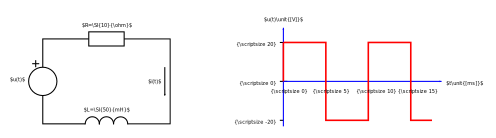
\includegraphics{Imatges/Cap-Fourier-Exemple-Circuit.pdf}
\end{figure}

 El per\'{\i}ode de la tensi\'{o} $u(t)$ \'{e}s: $T=10\unit{ms}$, i la
seva velocitat angular: $\omega = 2\pi/T = 200\pi\unit{rad/s}$;
matem\`{a}ticament, $u(t)$ s'expressa com:
\[
u(t) = \begin{cases} \rule{3.2mm}{0pt} 20\unit{V} & 0\unit{ms} < t < 5\unit{ms} \\
       -20\unit{V} & 5\unit{ms} \leq t \leq 10\unit{ms} \end{cases}
\]

Comencem calculant l'expansi\'{o} en s\`{e}rie de Fourier de la tensi\'{o}
$u(t)$. Aquesta funci\'{o} es senar i t\'{e} simetria de semiona, i per tant
 compleix: $u(t)=-u(-t)$ i $u(t) = -u(t+\frac{T}{2})$; com a
conseq\"{u}\`{e}ncia d'aix\`{o}, \'{u}nicament seran diferents de zero el
coeficients $B_n$ d'\'{\i}ndex senar $(B_1,B_3,B_5,\ldots)$. Donat que
$u(t)$ est\`{a} definida en dos trossos, calcularem els coeficients
$B_n$ segons:
\[
\begin{split}
    B_n &= \frac{2}{T} \left( \int_0^{T/2} u(t) \sin(n \omega t) +
    \int_{T/2}^{T} u(t) \sin(n \omega t) \right) =\\[0.5ex]
    &= 200 \left( \int_0^{5\cdot 10^{-3}} 20 \sin(200 n \pi t) +
    \int_{5\cdot 10^{-3}}^{10^{-2}} -20 \sin(200 n \pi t) \right) =\\[0.5ex]
    &= 200 \left( \left. -\frac{\cos(200 n \pi t)}{10 n \pi}\right|_0^{5\cdot 10^{-3}}
    +  \left.\frac{\cos(200 n \pi t)}{10 n \pi}\right|_{5\cdot
    10^{-3}}^{10^{-2}}\right)=\\[0.5ex]
    &= 200\left( \frac{1}{10 n \pi} - \frac{\cos n \pi}{5 n \pi} +
    \frac{\cos (2 n \pi)}{10 n \pi}\right)
    \qquad\qquad(n=1,3,5,\ldots)
\end{split}
\]

Si tenim en compte que per a valors senars de l'\'{\i}ndex $n$, es
compleix: $\cos n \pi = -1$ i $\cos (2 n \pi) = 1$, tenim:
\[
    B_n = 200 \left( \frac{1}{10 n \pi} - \frac{-1}{5 n \pi} +
    \frac{1}{10 n \pi} \right) = \frac{80}{n \pi}
    \qquad\qquad(n=1,3,5,\ldots)
\]

Aix\'{\i} doncs, l'expansi\'{o} en s\`{e}rie de Fourier de la tensi\'{o} $u(t)$ \'{e}s:
\[
    u(t) = \frac{80}{\pi} \left( \sin \omega t + \frac{\sin (3 \omega t)}{3} +
    \frac{\sin (5 \omega t)}{5} + \frac{\sin (7 \omega t)}{7} +
    \frac{\sin (9 \omega t)}{9} + \frac{\sin (11 \omega t)}{11} +\cdots\right)
\]

En el punt de discontinu\"{\i}tat $t=5\unit{ms}$, tenim:
\[
    u(5\cdot10^{-3}\unit{s}) =\frac{80}{\pi} \left( \sin \pi + \frac{\sin 3 \pi}{3} +
    \frac{\sin 5 \pi}{5} + \frac{\sin 7 \pi}{7} +
    \frac{\sin 9 \pi}{9} +\frac{\sin 11 \pi}{11}+\cdots\right) = 0\unit{V}
\]

Es comprova que en complir-se la condici\'{o} de Dirichlet, aquest valor
correspon al valor mitj\`{a} dels l\'{\i}mits esquerra (20) i dret (-20)  de
la funci\'{o} en aquest punt.

A continuaci\'{o} es pot veure la gr\`{a}fica de la tensi\'{o} $u(t)$, que
s'obt\'{e} utilitzant la seva expansi\'{o} en s\`{e}rie de Fourier, fins a la
component harm\`{o}nica d'\'{\i}ndex 11:
\begin{figure}[h]
\centering
    \includegraphics{Imatges/Cap-Fourier-Exemple-Tensio.pdf}
\end{figure}

La imped\`{a}ncia de la c\`{a}rrega formada per la resist\`{e}ncia $R$ i la
induct\`{a}ncia $L$, tindr\`{a} un valor $\cmplx{Z}_n$ diferent per a
cadascuna de les tensions fonamental i harm\`{o}niques presents en la
tensi\'{o} $u(t)$; els valors de $\cmplx{Z}_n$ per als primes \'{\i}ndex s\'{o}n:
\begin{alignat*}{3}
    \cmplx{Z}_1 &= R + \ju\, \omega L &&= (10 + \ju\cdot 200\cdot \pi\cdot 50\cdot 10^{-3})\unit{\ohm} &&=32{,}9691_{\measuredangle
    1{,}2626\unit{rad}}\unit{\ohm}\\
    \cmplx{Z}_3 &= R + \ju\, 3 \omega L &&= (10 + \ju\cdot 3\cdot 200\cdot \pi\cdot 50\cdot 10^{-3})\unit{\ohm} &&=94{,}7768_{\measuredangle
    1{,}4651\unit{rad}}\unit{\ohm}\\
    \cmplx{Z}_5 &= R + \ju\, 5 \omega L &&= (10 + \ju\cdot 5\cdot 200\cdot \pi\cdot 50\cdot 10^{-3})\unit{\ohm} &&=157{,}3976_{\measuredangle
    1{,}5072\unit{rad}}\unit{\ohm}\\
    \cmplx{Z}_7 &= R + \ju\, 7 \omega L &&= (10 + \ju\cdot 7\cdot 200\cdot \pi\cdot 50\cdot 10^{-3})\unit{\ohm} &&=220{,}1387_{\measuredangle
    1{,}5254\unit{rad}}\unit{\ohm}\\
    \cmplx{Z}_9 &= R + \ju\, 9 \omega L &&= (10 + \ju\cdot 9\cdot 200\cdot \pi\cdot 50\cdot 10^{-3})\unit{\ohm} &&=282{,}9201_{\measuredangle
    1{,}5354\unit{rad}}\unit{\ohm}\\
    \cmplx{Z}_{11} &= R + \ju\, 11 \omega L &&= (10 + \ju\cdot 11\cdot 200\cdot \pi\cdot 50\cdot 10^{-3})\unit{\ohm} &&=345{,}7198_{\measuredangle
    1{,}5419\unit{rad}}\unit{\ohm}
\end{alignat*}

L'expansi\'{o} en s\`{e}rie de Fourier del corrent $i(t)$ ser\`{a} an\`{a}loga a la
de la tensi\'{o} $u(t)$, \'{e}s a dir, tan sols tindr\`{a} funcions sinus
d'\'{\i}ndex senar. Donat que la c\`{a}rrega \'{e}s inductiva, cadascun dels
termes del corrent estar\`{a} endarrerit respecte del terme corresponent
de la tensi\'{o}, en un valor indicat per l'argument de cada imped\`{a}ncia.
El valor de pic de cada terme del corrent $\hat{I}_n$, s'obt\'{e}
dividint el valor de pic de cada terme de la tensi\'{o} $\hat{U}_n$ pel
m\`{o}dul de la imped\`{a}ncia corresponent; els valors de $\hat{I}_n$ per
als primes \'{\i}ndex s\'{o}n:
\begin{align*}
    \hat{I}_1 &= \frac{\hat{U}_1}{|\cmplx{Z}_1|} = \frac{80\unit{V}}{\pi\cdot32{,}9691\unit{\ohm}} = 0{,}7724\unit{A}
    & \hat{I}_3 &= \frac{\hat{U}_3}{|\cmplx{Z}_3|} =\frac{80\unit{V}}{3\cdot\pi\cdot 94{,}7768\unit{\ohm}} = 0{,}0896\unit{A}\\[0.5ex]
    \hat{I}_5 &= \frac{\hat{U}_5}{|\cmplx{Z}_5|} =\frac{80\unit{V}}{5\cdot\pi\cdot 157{,}3976\unit{\ohm}} =0{,}0324\unit{A}
    & \hat{I}_7 &= \frac{\hat{U}_7}{|\cmplx{Z}_7|} =\frac{80\unit{V}}{7\cdot\pi\cdot 220{,}1387\unit{\ohm}} =
    0{,}0165\unit{A}\\[0.5ex]
    \hat{I}_9 &= \frac{\hat{U}_9}{|\cmplx{Z}_9|} =\frac{80\unit{V}}{9\cdot\pi\cdot 282{,}9201\unit{\ohm}} =
    0{,}0100\unit{A} & \hat{I}_{11} &= \frac{\hat{U}_{11}}{|\cmplx{Z}_{11}|} =\frac{80\unit{V}}
    {11\cdot\pi\cdot 345{,}7198\unit{\ohm}} =  0{,}0067\unit{A}
\end{align*}

Amb aquests valor calculats, l'expansi\'{o} en s\`{e}rie de Fourier del
corrent $i(t)$ \'{e}s:
\[\begin{split}
     i(t) &=  0{,}7724 \sin(\omega t - 1{,}2626) +  0{,}0896 \sin(3 \omega t -
     1{,}4651) + 0{,}0324 \sin(5 \omega t - 1{,}5072) +{}\\
     &+ 0{,}0165 \sin(7 \omega t - 1{,}5254) + 0{,}0100 \sin(9 \omega t - 1{,}5354)
     +0{,}0067 \sin(11 \omega t - 1{,}5419) +\cdots
\end{split}\]

A continuaci\'{o} es pot veure la gr\`{a}fica del corrent $i(t)$, que s'obt\'{e}
utilitzant la seva expansi\'{o} en s\`{e}rie de Fourier, fins a la component
harm\`{o}nica d'\'{\i}ndex 11:

\begin{figure}[h]
\centering
  \includegraphics{Imatges/Cap-Fourier-Exemple-Corrent.pdf}
\end{figure}

Calculem a continuaci\'{o} el valor efica\c{c} $I$ del corrent:
\[\begin{split}
    I &= \sqrt{\left(\tfrac{0{,}7724}{\sqrt{2}}\unit{A}\right)^2 +
        \left(\tfrac{0{,}0896}{\sqrt{2}}\unit{A}\right)^2 +
        \left(\tfrac{0{,}0324}{\sqrt{2}}\unit{A}\right)^2 +
        \left(\tfrac{0{,}0165}{\sqrt{2}}\unit{A}\right)^2 +
        \left(\tfrac{0{,}0100}{\sqrt{2}}\unit{A}\right)^2 +
        \left(\tfrac{0{,}0067}{\sqrt{2}}\unit{A}\right)^2 \cdots}
        \,\approx \\[1ex]
        &\approx 0{,}5505\unit{A}
\end{split}\]

Finalment, la pot\`{e}ncia $P$ dissipada en la resist\`{e}ncia ser\`{a}:
\[
    P = R I^2 \approx 10\unit{\ohm} \cdot (0{,}5505\unit{A})^2 =
    3{,}03\unit{W}
\]

Aquest valor tamb\'{e} es pot calcular a partir de l'equaci\'{o}
\eqref{eq:pot_fu}. La pot\`{e}ncia aix\'{\i} calculada, correspon a la
pot\`{e}ncia activa cedida per la font de tensi\'{o}, i donat que la
resist\`{e}ncia $R$ \'{e}s l'\'{u}nic component del circuit que en consumeix,
aquest m\`{e}tode ens proporcionar\`{a} el mateix resultat; utilitzant les
expansions en s\`{e}rie de Fourier de la tensi\'{o} $u(t)$ i del corrent
$i(t)$, fins a la component harm\`{o}nica d'\'{\i}ndex 11, tenim:
\[\begin{split}
    P &\approx U_1 I_1 \cos\varphi_1 +  U_3 I_3 \cos\varphi_3 +
     U_5 I_5 \cos\varphi_5 +{}\\[0.7ex]
     &+  U_7 I_7 \cos\varphi_7 +
     U_9 I_9 \cos\varphi_9 + U_{11} I_{11} \cos\varphi_{11} ={}
\end{split}\]


\[\begin{split}
    &= \frac{80}{\pi\cdot\sqrt{2}}\unit{V} \cdot
    \frac{0{,}7724}{\sqrt{2}}\unit{A} \cdot \cos 1{,2626} +
    \frac{80}{3\cdot\pi\cdot\sqrt{2}}\unit{V} \cdot
    \frac{0{,}0896}{\sqrt{2}}\unit{A} \cdot \cos 1{,4651} + {} \\[0.7ex]
    &+ \frac{80}{5\cdot\pi\cdot\sqrt{2}}\unit{V} \cdot
    \frac{0{,}0324}{\sqrt{2}}\unit{A} \cdot \cos 1{,5072} +
    \frac{80}{7\cdot\pi\cdot\sqrt{2}}\unit{V} \cdot
    \frac{0{,}0165}{\sqrt{2}}\unit{A} \cdot \cos 1{,5254} + {}\\[0.7ex]
    &+ \frac{80}{9\cdot\pi\cdot\sqrt{2}}\unit{V} \cdot
    \frac{0{,}0100}{\sqrt{2}}\unit{A} \cdot \cos 1{,5354} +
    \frac{80}{11\cdot\pi\cdot\sqrt{2}}\unit{V} \cdot
    \frac{0{,}0067}{\sqrt{2}}\unit{A} \cdot \cos 1{,5419}= {}\\[0.7ex]
    &=3{,}03\unit{W}
\end{split}\]

En la resoluci\'{o} d'aquest exemple, hem emprat tan sols els sis
primers termes de las s\`{e}ries de Fourier de la tensi\'{o} i del corrent;
no obstant, el valor  obtingut de la pot\`{e}ncia ha de ser prou prec\'{\i}s, ja que
els valors de pic dels termes de la s\`{e}rie del corrent, disminueixen de
valor r\`{a}pidament.

Refarem a continuaci\'{o} els c\`{a}lculs utilitzant m\'{e}s termes, amb l'ajut
del programa
\textit{Mathematica}${}^\circledR$.
\index{Mathematica@\textit{Mathematica}${}^\circledR$}
Definim en primer lloc el valor de pic de cada
 terme de la tensi\'{o} i el valor del m\`{o}dul de la imped\`{a}ncia corresponent,
calculem a continuaci\'{o} els 100 primers termes del corrent de pic, i
per acabar calculem el valor efica\c{c} del corrent i la pot\`{e}ncia:
\begin{alltt}
\bfseries\small In[1]:= u[n_] = 80 / (Pi (2n-1));\\
 In[2]:= z[n_] = Abs[10 + I (2n-1) 200 Pi 50 10^-3];\\
 In[3]:= i = Table[u[n], \{n, 1, 100\}] / Table[z[n], \{n, 1, 100\}];\\
 In[4]:= Irms = Sqrt[Apply[Plus, (i/Sqrt[2])^2]] // N\\
Out[4]:= 0.550511\\
 In[5]:= P = 10 Irms^2\\
Out[5]:= 3.03063
\end{alltt}

Tamb\'{e} podem fer aquests c\`{a}lculs amb el programa
MATLAB${}^\circledR$, tal com es veu a continuaci\'{o}:
\index{MATLAB@\textit{MATLAB}${}^\circledR$}
\begin{alltt}
\bfseries\small>> u = 80./(pi*(2*[1:1:100]-1));\\
>> z = abs(10 + i*(2*[1:1:100]-1)*200*pi*50*1e-3);\\
>> i = u./z;\\
>> Irms = sqrt(sum((i./sqrt(2)).^2))\\
Irms =\\
    0.5505\\
>> P = 10*Irms^2\\
P =\\
    3.0306
\end{alltt}

 Com es pot observar, el valor de la pot\`{e}ncia obtingut amb qualsevol dels dos
 programes,
 coincideix d'una manera prou aproximada, amb el valor calculat a m\`{a}
anteriorment.
\end{exemple}
